\documentclass[11pt,a4paper]{article}
\PassOptionsToPackage{obeyspaces,spaces}{url}
\usepackage{fontspec,unicode-math}
\setmainfont{texgyrepagella-regular.otf}[BoldFont=texgyrepagella-bold.otf,ItalicFont=texgyrepagella-italic.otf,BoldItalicFont=texgyrepagella-bolditalic.otf]
\setmathfont{texgyrepagella-math.otf}
\setmonofont{DejaVuSansMono.ttf}[Scale=0.8,BoldFont=DejaVuSansMono-Bold.ttf]
\usepackage[margin=2.2cm]{geometry}
\usepackage{booktabs,array,enumitem,xcolor,url,microtype,tikz,slashed,listings}
\lstset{basicstyle=\ttfamily\footnotesize, escapechar=@, breaklines=true, columns=fullflexible,
  keepspaces=true, frame=single, rulecolor=\color{gray!50}, xleftmargin=4pt, framexleftmargin=4pt,
  commentstyle=\color{gray}, morecomment=[l]{--}, extendedchars=false, aboveskip=6pt, belowskip=6pt}
\usetikzlibrary{positioning,arrows.meta,fit,backgrounds,calc,shapes.geometric}
\usepackage[colorlinks=true,linkcolor=blue!50!black,urlcolor=blue!50!black]{hyperref}
\makeatletter\g@addto@macro{\UrlBreaks}{\do\_\do\.\do\-}\makeatother
\newcommand{\lean}[1]{{\footnotesize\ttfamily\nolinkurl{#1}}}
\newcommand{\file}[1]{{\small\ttfamily\nolinkurl{#1}}}
\pdfstringdefDisableCommands{\def\lean#1{#1}\def\file#1{#1}\def\nolinkurl#1{#1}}
\setlength{\parskip}{4pt}
\emergencystretch=2em

\definecolor{hand}{RGB}{214,120,60}
\definecolor{table}{RGB}{50,120,190}
\definecolor{gen}{RGB}{70,150,90}
\definecolor{plan}{RGB}{140,90,170}

\tikzset{
  box/.style={draw, rounded corners=2pt, align=center, font=\small, inner sep=4pt, minimum height=7mm, text width=#1},
  box/.default=30mm,
  handb/.style={box=#1, draw=hand, fill=hand!8},
  handb/.default=30mm,
  tableb/.style={box=#1, draw=table, fill=table!8},
  tableb/.default=30mm,
  genb/.style={box=#1, draw=gen, fill=gen!8},
  genb/.default=30mm,
  planb/.style={box=#1, draw=plan, fill=plan!8, dashed},
  planb/.default=30mm,
  arr/.style={-{Latex[length=2mm]}, thick},
  eq/.style={{Bar}-{Bar}, thick, densely dotted},
  lab/.style={font=\scriptsize, fill=white, inner sep=1pt},
  grp/.style={draw, rounded corners=4pt, inner sep=6pt, font=\footnotesize\bfseries, dashed, gray!70},
}

\title{The design of \texttt{GaugeTheory/}}
\author{Jinzheng Li}
\date{Draft for discussion, 22 September 2026}

\begin{document}
\maketitle

\section{Purpose}

\lean{Physlib/ClassicalFieldTheory/GaugeTheory/} is the symbolic framework for the local content of a gauge theory: the algebra in which a Lagrangian is written, the gauge and Lorentz actions on it, and the invariants of a given mass dimension. Fields enter only through their \emph{jets} at one point, the formal symbols $\partial_s\psi_\alpha$; there is no spacetime, no integral and no equation of motion.

The folder is organised by one rule. \textbf{Every layer takes a datum and returns constructions and theorems; a concrete theory contributes only its data.} The Standard Model is a gauge group named as a list of factors and a table of fields; everything else about it is inherited.

The layers are cut by level of generality only: a gauge datum, one species, a content of species, the algebra of a content, and its covariant subalgebra. There is one notion of species, of which matter fields and the connection are instances, and one algebra tower, of which the pure gauge theory and the sectors are instances. This note records the intended structure, as a basis for discussion and, later, for a paper. Names in it are the intended ones; the present tree differs from it, and \S7 maps the two onto each other. Open choices are collected in \S6.

\section{The idea}

\begin{itemize}
\item \textbf{Jets.} With $\mathtt{JetRing} = \mathbb C[[x_0,x_1,x_2,x_3]]$, the jet of a field valued in $V$ is an element of $\mathtt{JetRing}\otimes V$; $\partial_\mu$ acts on the series, evaluation takes the constant coefficient.
\item \textbf{Gauge jets.} A gauge transformation is replaced by its jet $U$ in a jet group $G_J$, with value $\mathrm{eval}\,U\in G_0$, Lie algebra $\mathfrak g_J$, derivatives, adjoint action and Maurer--Cartan form $\omega_\mu(U) = i(\partial_\mu U)U^{-1}$. These maps and their laws form the gauge datum; nothing downstream knows which group it is.
\item \textbf{Species.} A species is a finite-dimensional $V$ with a Lorentz representation, a parity, a mass weight, and an \emph{affine} action of $G_J$ on $\mathtt{JetRing}\otimes V$: a linear part $\ell(U)$ and a translation $t(U)$ with $t(UV) = t(U) + \ell(U)\,t(V)$. A matter field has $t = 0$ and $\ell$ fibrewise, generated by an infinitesimal action of $\mathfrak g$. The connection has $\ell = \mathrm{Ad}$ and $t = \omega$, so that $A_\mu\mapsto \mathrm{Ad}_U A_\mu + \omega_\mu(U)$.
\item \textbf{The algebra.} A content $T$ is a finite family of species containing the connection. Its local field algebra $J(T)$ is the free graded-commutative algebra on the symbols $\partial_s\psi^\alpha$ of all species (exterior on the odd ones, symmetric on the even ones). Every action on $J(T)$ is defined by its values on generators and extended by the universal property; the translation part of a species' law is the inhomogeneous term of its generators. Reality is a star structure on $J(T)$: conjugation swaps a matter symbol with its conjugate and fixes the connection.
\item \textbf{Functoriality.} An inclusion of contents $S\subseteq T$ gives an injective equivariant algebra map $J(S)\to J(T)$ with a retraction. Sectors are its images; the pure gauge theory is $J$ of the content consisting of the connection alone.
\item \textbf{Invariants.} Mass weight is twice the mass dimension (derivative 2, scalar 2, Weyl fermion 3, connection 2). The Lagrangian of dimension four is the submodule of gauge and Lorentz invariants of weight at most 8. On the covariant subalgebra the jet action factors through $G_0$, so the classification is ordinary invariant theory, sector by sector.
\end{itemize}

\section{The layers}

\begin{center}
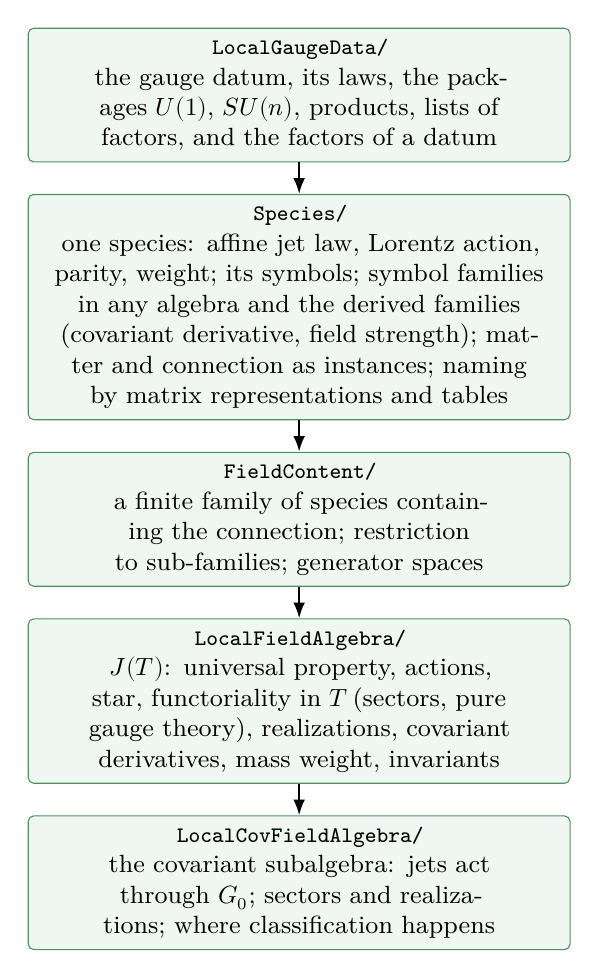
\begin{tikzpicture}[node distance=4mm and 8mm]
  \node[genb=66mm] (lgd) {\lean{LocalGaugeData/}\\ the gauge datum, its laws, the packages $U(1)$, $SU(n)$, products, lists of factors, and the factors of a datum};
  \node[genb=66mm, below=of lgd] (sp) {\lean{Species/}\\ one species: affine jet law, Lorentz action, parity, weight; its symbols; symbol families in any algebra and the derived families (covariant derivative, field strength); matter and connection as instances; naming by matrix representations and tables};
  \node[genb=66mm, below=of sp] (fc) {\lean{FieldContent/}\\ a finite family of species containing the connection; restriction to sub-families; generator spaces};
  \node[genb=66mm, below=of fc] (lfa) {\lean{LocalFieldAlgebra/}\\ $J(T)$: universal property, actions, star, functoriality in $T$ (sectors, pure gauge theory), realizations, covariant derivatives, mass weight, invariants};
  \node[genb=66mm, below=of lfa] (lcfa) {\lean{LocalCovFieldAlgebra/}\\ the covariant subalgebra: jets act through $G_0$; sectors and realizations; where classification happens};
  \draw[arr] (lgd) -- (sp); \draw[arr] (sp) -- (fc); \draw[arr] (fc) -- (lfa); \draw[arr] (lfa) -- (lcfa);
\end{tikzpicture}
\end{center}

Imports go down the line only. Each layer exposes one structure as its datum and proves everything for an arbitrary instance of it.

\subsection{\lean{LocalGaugeData/}: the gauge datum}

\emph{Input:} none. \emph{Output:} the structure \lean{LocalGaugeData G₀ }$\mathfrak g$\lean{ GJ }$\mathfrak g$\lean{J} and its instances.

\begin{itemize}
\item The structure: \lean{eval}, \lean{ofConstant}, their Lie versions, \lean{deriv}, \lean{coord}, \lean{adjoint}, \lean{maurerCartan}, and the laws (cocycle, structure equation, Leibniz for the adjoint).
\item What follows from the laws alone: the Taylor--Leibniz theorem for the adjoint coefficients, the symmetrised Maurer--Cartan form, the truncation filtration, the classes \lean{Faithful} (a jet is determined by its Taylor data) and \lean{Free} (every Taylor family occurs).
\item The packages \lean{u1}, \lean{su n}, \lean{prod}, and \lean{ofFactors} for a list of symbols such as \lean{[.SU 3, .SU 2, .U1]}.
\item The factors of a datum, a $U(1)$ or $SU(n)$ projection out of it (\lean{U1Factor}, \lean{SUFactor}, \lean{Factors}). They describe the gauge datum, not matter, so they live here.
\end{itemize}

\subsection{\lean{Species/}: one species}

\emph{Input:} a gauge datum. \emph{Output:} the structure \lean{Species jets} and the two ways to build one.

\begin{itemize}
\item The structure: $V$, \lean{repLorentz}, \lean{parity}, \lean{massWeight}, and the affine jet law (linear part, translation, cocycle law). Its symbols form the jet component space, with the Lorentz action, the derivative, the weight scaling and the induced affine action on symbols.
\item Symbol families: a family of elements of an algebra $B$ indexed by derivative multisets and covectors of $V$ \emph{transforms as the species} when each symbol transforms by the Leibniz convolution of the species' Taylor coefficients, plus the translation. This is the single law that today is \lean{TransformsIn} for matter and \lean{GaugeAlgebraRealization} for the connection.
\item Matter species, \lean{Species.ofRep}: translation zero, linear part a fibrewise representation, together with the infinitesimal action that generates it (\lean{IsInfinitesimalActionOf}). Derived family: the covariant derivative $\nabla_\rho F=[\partial_\rho F]+A_\rho\cdot F$ of a family in any algebra carrying the connection, and the theorem that it transforms as the species.
\item The connection species, \lean{Species.connection jets}: value space $\text{CoVector}\otimes\mathfrak g$, adjoint linear part, Maurer--Cartan translation, weight 2. Derived family: the field strength and its covariant derivatives, and the generation theorem, that the connection symbols are generated by symmetrised derivatives together with covariant derivatives of the field strength.
\item Naming, \lean{MatrixRep/}: a matrix of jets with its action matrices and two identities yields a matter species; the fundamental of an $SU(n)$ factor, charge twists, trivial, Kronecker and conjugate representations; and the table vocabulary, where a Lorentz label and a charge tuple such as \lean{(.L, .singlet, .fund, -3)} name a species.
\end{itemize}

\subsection{\lean{FieldContent/}: a content}

\emph{Input:} a gauge datum. \emph{Output:} the structure \lean{FieldContent jets}: a finite species type, a species for each, and the connection among them.

\begin{itemize}
\item The generator space of a content, the sum of the jet component spaces of its species, graded by parity, with the species-wise Lorentz action, affine jet action and weight scaling.
\item Restriction: a sub-family of a content is a content, and the connection-only content is the minimum.
\item The properties a content may have: \lean{PureJetsActTrivially} (a jet with trivial value acts trivially at the base point) and \lean{GaugeLorentzCompatible} (the infinitesimal action commutes with the Lorentz action). A content compiled from a table (\lean{toFieldContent}) has the second.
\end{itemize}

\subsection{\lean{LocalFieldAlgebra/}: the algebra of a content}

\emph{Input:} a content $T$. \emph{Output:} $J(T)$ and its structure.

\begin{itemize}
\item The universal property: an assignment of the generators lifts uniquely to an algebra map, with the Koszul sign for odd generators.
\item The gauge and Lorentz actions, defined on generators from the species laws and extended by lift; the star structure. The symbol families of each species transform as the species, by construction.
\item Functoriality: for $S\subseteq T$ the map $J(S)\to J(T)$ is injective and equivariant, with the retraction that sends the other generators to zero. Sectors are the images of sub-contents; the gauge sector is the image of the connection-only content.
\item Realizations: equivariant algebra maps $J(T)\to B$, which are the same as families in $B$ transforming as the species of $T$; restriction along $S\subseteq T$.
\item The covariant derivatives of all species inside $J(T)$, and the field strength.
\item Mass weight: the scaling by $c$, the graded pieces, the filtration \lean{massWeightSubmoduleLE w}, the invariants \lean{gaugeInvariants}, \lean{lorentzInvariants}, \lean{invariantsLE}, and their transport along isomorphisms respecting the actions and the scaling.
\end{itemize}

\subsection{\lean{LocalCovFieldAlgebra/}: the covariant subalgebra}

\emph{Input:} a content with the two properties above. \emph{Output:} the subalgebra of $J(T)$ generated by the covariant towers of all species and of the field strength. Jets act on it through $G_0$, so its gauge invariants are the invariants of the ordinary group; it has the sectors and realizations of $J(T)$, restricted. Every classification theorem is proved here and transported to $J(T)$.

\section{What a model sees}

A model is a card: a list of factors and a table.
\begin{lstlisting}
abbrev gauge : List FactorSpec := [.SU 3, .SU 2, .U1]
noncomputable abbrev gaugeData := ofFactors gauge
abbrev leptonDoublet : SpeciesData factors := (.L, .singlet, .fund, -3)
...
noncomputable def content : FieldContent gaugeData := table.toFieldContent
\end{lstlisting}
Below the card there are no further definitions. A species of the model is an abbreviation of the value space its datum produces; its actions are projections of the species. A theorem about the model is stated only in the card and the generic vocabulary, as in
\begin{lstlisting}
theorem invariantsLE_four (x : content.LocalFieldAlgebra) :
    (x @$\in$@ content.massWeightSubmoduleLE 4
        @$\wedge$@ (@$\forall$@ U : Factors.G gauge, content.repJet U x = x)
        @$\wedge$@ @$\forall$@ @$\Lambda$@ : SL(2,@$\mathbb C$@), content.repLorentzGroup @$\Lambda$@ x = x)
      @$\leftrightarrow$@ x @$\in$@ @$\mathbb C$@ @$\cdot$@ 1 @$\sqcup$@ @$\mathbb C$@ @$\cdot$@ higgsMass
\end{lstlisting}
so that reading the statement requires only the card and this note.

\section{Design rules}

\begin{enumerate}
\item Data in, theorems out. A layer exposes one structure as its datum and proves everything for an arbitrary instance. No file in \lean{GaugeTheory/} mentions a particular gauge group or content.
\item Imports go down the line of \S3. In particular the gauge datum does not import species, and species do not import contents.
\item One notion at each level. Matter fields and the connection are species; the pure gauge theory and the sectors are contents; there is one algebra tower. Nothing is built twice and identified afterwards.
\item Constructions on free algebras go through the universal property. An action is its assignment on generators; a law is an equality of lifts; a realization is an equivariant assignment.
\item Indices are covectors, never basis indices: the adjoint index of $A_\mu$ is $\varphi\in\mathfrak g^*$, the value index of a species is $\varphi\in V^*$. Bases appear only in the naming layer.
\item A concrete theory adds a card and proofs. A missing generic notion is added to its layer, not to the model.
\end{enumerate}

\section{Questions for discussion}

\begin{enumerate}
\item \textbf{One species structure or two.} The affine law makes matter and the connection instances of one structure, at the price of a translation field that is zero for every matter species. The alternative keeps \lean{MatterField} and the connection separate and states the symbol-family law twice. Is the uniformity worth the extra field?
\item \textbf{Real or complex tower.} The connection is real and its algebra is real today. The single tower is complex, with reality as a star structure. Does anything downstream (the gauge-sector classification, the reality of the Lagrangian) need the real algebra as an object, rather than the star?
\item \textbf{The connection in the content.} Today the connection is implicit: every content has it because every gauge datum has it. Making it an explicit member of the family makes restriction and the connection-only content ordinary, but every content then carries a species that is not chosen. Explicit or implicit?
\item \textbf{Sectors by functoriality.} Deriving sectors from inclusions of contents removes four files of identifications, but restriction along $S\subseteq T$ has to be an honest map of contents, which fixes how species are indexed (a subtype of the species type). Is that indexing acceptable to the existing sector proofs?
\item \textbf{Names.} \lean{Species}, \lean{FieldContent} against the current \lean{MatterField}, \lean{GaugeFieldData}; \lean{content} against \lean{fieldData} in a card. Renaming is cheap now and expensive later.
\item \textbf{Order of work.} Steps 1 and 2 of \S7 can go into PR \#1415 or follow it; steps 3 and 4 touch the gauge-boson code and the Standard Model classification and need their owners. Which of them, if any, should precede the remaining Standard Model migration?
\end{enumerate}

\section{Distance from the current tree}

The current tree has six folders. Their contents map onto the five above as follows.

\begin{center}\small
\begin{tabular}{@{}p{62mm}p{92mm}@{}}
\toprule
current & intended \\
\midrule
\lean{LocalGaugeData/} & \lean{LocalGaugeData/}, plus the factor types now in \lean{MatterField/MatrixRep/Factors} \\
\lean{MatterField/} & \lean{Species/} (matter instance, covariant derivative, \lean{MatrixRep/}, table) \\
\lean{GaugeBoson/Basic}, \lean{GaugeBoson/Realization/} & \lean{Species/} (connection instance, field strength, generation theorem) \\
\lean{GaugeBoson/LocalGaugeFieldAlgebra/} & \lean{LocalFieldAlgebra/} at the connection-only content \\
\lean{GaugeBoson/LocalGaugeCovFieldAlgebra/} & \lean{LocalCovFieldAlgebra/} at the connection-only content \\
\lean{GaugeFieldData/} & \lean{FieldContent/}, with the connection made explicit \\
\lean{LocalFieldAlgebra/}, \lean{LocalCovFieldAlgebra/} & the same, with sectors derived from functoriality \\
\bottomrule
\end{tabular}
\end{center}

The concrete differences, in the order they should be removed:
\begin{enumerate}
\item \lean{LocalGaugeData/} imports matter: the factor types live in \lean{MatterField/MatrixRep/}, and \lean{TransformsIn}, \lean{InfinitesimalAction} import \lean{MatterField/CovariantDeriv} and \lean{LocalFieldAlgebra/JetRep}. Move the factor types down and the two files into the species layer.
\item Matter and the connection have different shapes of API: \lean{MatterField} with \lean{TransformsIn} against \lean{GaugeBoson} with \lean{GaugeAlgebraRealization}. Introduce the affine species structure with both as instances, and state the symbol-family law once.
\item Sectors are built by hand and the gauge sector is identified with a separately built algebra (four \lean{GaugeSector} files). Prove functoriality of $J$ in the content and derive them.
\item The connection has its own algebra tower, real, of about 3300 lines. Replace it by the connection-only content, and record reality by the star structure. This is last, because the Standard Model's gauge-sector classification is built on that tower.
\end{enumerate}
Steps 1 and 2 are cleanup. Steps 3 and 4 change conventions shared with the existing code and should be proposed on Zulip before they are started.

Independently of the folder structure, the Standard Model still has five species built by hand alongside its card, its classification theorems are stated on the hand-built datum, and the generic term constructors, a unitarity field on matrix representations and generic anomaly coefficients are not yet in the library.

\end{document}
